\documentclass[11pt, english]{article}

\usepackage{multicol}
\usepackage{hyperref}
\usepackage[eng]{felipito}
\usepackage{stfloats}
\usepackage{mathpazo}

\usepackage[margin=0.8in, left=0.7in, right=0.7in]{geometry}

\graphicspath{{./Graphics/}}

% Colors
\definecolor{urlcolor}{rgb}{0,.145,.698}
\definecolor{linkcolor}{rgb}{.71,0.21,0.01}
\definecolor{citecolor}{rgb}{.12,.54,.11}


% Document title
\title{\bf Problem Set 4 \\ Statistics, Computation and
Applications\\[-1ex]}
\author{Felipe del Canto}
\date{November, 2021}
    
\hypersetup{
	breaklinks=true,  % so long urls are correctly broken across lines
    colorlinks=true,
    urlcolor=urlcolor,
    linkcolor=linkcolor,
    citecolor=citecolor,
}

\begin{document}
    
\maketitle
   
\begin{multicols}{2}

\section*{Problem 4.1: Suggesting Similar\\ Papers}

For part (a), let $N$ be the number of papers, $C$ be adjacency matrix for the citation network, and let $\gamma$ be the adjacency matrix for the co-citation network. Observe that papers $i$ and $j$ are co-cited with weight $w$ if and only if there are $w$ papers such that $C^{T}(i,k) \cdot C(k,j) = 1$ for each paper $k \in \{1,\ldots,w\}$. Indeed, if $i$ and $j$ are co-cited with weight $w$, then there exist $w$ papers such that $C(k,i) = C(k,j) = 1$ for each $k \in \{1, \ldots, w\}$. This implies that $C^{T}(i,k) \cdot C(k,j) = 1$ for each one. Conversely, if there are $w$ papers with $C^{T}(i,k) \cdot C(k,j) = 1$ for each $k \in \{1, \ldots, w\}$, then $C(k,i) = C(k,j)$ and, consequently, papers $i$ and $j$ are co-cited with weight $w$. The previous claim shows that a first attempt at obtaining the co-citation adjacency matrix is
	$$\gamma = C^{T}C.$$
Since $C^{T}$ codes the directed edges from the cited papers from the one that cites them, then the product $C^{T}C$ counts the 2-step directed edges between two papers that are cited by the same third paper. Since a paper is co-cited with itself the number of times another paper cite it, this product also captures it. Consequently, the previous equality is the desired computation.

For part (b), the process is similar to part (a), but focused on the papers that cite, instead of those cited. Now, we are interested in the two-step directed edges between to papers that cite the same paper. Consequently, if $\beta$ is the bibliographic coupling adjacency matrix, then the first approach should be
	$$\beta = CC^{T}.$$
This product captures the two-step directed edges that start in a citing paper and finish in another citing paper. Note that this product also captures the bibliography coupling between a paper and itself. Since a paper is bibliography coupled with itself with weight equal to the number of other papers it cites, then there are that same amount of two-step directed edges between a that paper and itself.

For part (c), consider two papers belonging to two different disciplines which described two different techniques. In principle, this papers are very different. Suppose, additionally, that these techniques are widely used in a third discipline and, consequently, their respective papers are usually cited by many articles belonging to this latter field. Under these assumptions, both of these papers will have a high co-citation weight, despite not dealing with a related subject. In contrast, their bibliographic coupling should be close (or equal) to zero. Evidently, a scientist writing a paper in the third discipline, will benefit much from knowing these two papers are used together in other articles related to the ones she is writing. However, this does not imply that the two papers are related. Instead, it shows that the research made by this scientist is related to the other work in her discipline. In contrast, consider two survey papers in some particular field, but one of them was published a few years before the other. Since these are surveys, their bibliographic coupling might be large, but since newer papers would tend to cite the most recent survey, their co-cite weight will be close to zero.

To answer which measure is more appropriate to indicate similarities, the first step would be to address in which sense we are considering two articles to be similar. If we are interested in determining the boundaries of a field, it might me more useful to rely on the bibliographic coupling. Since an author interested in inserting her work into a given field would likely cite many of its relevant articles, it is likely that papers belonging to a given field have many of their references in common. Observe that a similar argument could be done for the co-cite similarity. If two papers belong to a certain field, it is more likely they appear together in other bibliographies. However, the caveat is that the co-cite similarity is very sensitive to the year in which each paper is published. Two recent papers have not had the chance to be included in many bibliographies, making this similarity very sparse for recent articles. What is more, the co-cite similarity is in fact monotone non-decreasing with respect to time, whereas the bibliographic coupling is independent of time.

Now consider that, instead, a researcher is interested in determining which articles should she review before writing about a certain topic. In particular, she is following a certain paper and would like to know which other papers she should review. In this case, looking at similar papers using the bibliographic coupling could be a bad measure for two main reasons. First, each article's bibliography is an endogenous product. The author(s) of the main paper she is following chose carefully which citations they wanted to use, and other papers that share them may not be as useful for this new task. Second, bibliographies are often extensive and only contain limited amounts of information of each of their references. Consequently, the list of similar articles using the bibliographic coupling may be sparse. If, instead, the researcher could access which papers where co-cited with her main reference, then the work may be easier. A higher co-cite similarity implies that many independent authors linked her meaningful reference with other works she may use. This process is exogenous and typically does not depend on the author of the initial paper.

\section*{Problem 4.2: Co-offending Network}

\textit{Note: The dataset provided for this question has been altered in such a way that is is unrecognizable from the original.}\vspace{1.5ex}

The original dataset contains 1,4565,786 observations, each at the \texttt{offender\_id}-\texttt{event\_id}-\texttt{crime\_code} level. This is, each observation is a unique person, arrested at a given crime event, and charged with a given crime. Note that at any given crime event, the offender can be charged several different crimes. Within, the number of unique offenders is 538,851, and the number of different crime events are 1,163,423, which occurred between 1997 and 2004, according to \Cref{tab:crimes-per-year}. 

In terms of crimes, there is a total of 301 different crime codes. The 5 crimes that occurred the the most are shown in \Cref{tab:notorious-crimes}. Together, they comprise a total of 516,876 perpetrators, and correspond to, approximately, 35\% of the sample. In terms of crimes in general, there is high variability. Moreover, a great number of crimes have low occurrences, as can be seen in \Cref{fig:total-offenses-per-crime-full}. To gain more insight, the sample is restricted to crimes with less or equal than 5,000 offenders. For reference, the average number of offenders per crime is, approximately, 4,869. With this, of the 294 different codes, 254 (86.3\%) remain. The result can be seen in \Cref{fig:total-offenses-per-crime-small}. The plot changes slightly. Most of the codes have little offenders and, among the rest, there is high variability.

In terms of location, these five most notorious crimes occur mainly in county 682. This could be due to 682 being the most populated county in the database. The details can be found in \Cref{tab:notorious-crimes-county}. The table shows that, for crime 131, this county accounts for 84,952 offenders. This corresponds to, approximately, 78.63\% of all offenders arrested for this crime. The rest of the crimes present a share in county 684 that is large, but much smaller than for crime 131, round between 20\% and 29\%. To further see the relevance of this county, \Cref{tab:notorious-crimes-uniform-distribution} shows, for each crime, in how many different counties it was detected. Additionally, the table shows the contribution each county should have if crimes occurred evenly in each one. This contribution is computed as follows:
  $$ \text{Contribution}_{\,\text{crime}} = \frac{100}{\text{\# Different counties}_{\,\text{crime}}} $$
This table shows how concentrated is the distribution of crimes in county 682. In particular, it can be seen that crime 131 is present in almost a half of counties in which the rest of the crimes are. This can explain the abrupt jump in contribution in \Cref{tab:notorious-crimes-county}. 

Now, to create the co-offending network, the library \texttt{networkx} is used. This Python library is useful to compute metrics in an efficient way. Before using this module, the first step is to create the adjacency matrix, using \texttt{scipy}'s sparse matrix class. First, the complete network, including solo offenders is created. A solo offender is a person whose only neighbor in the network is himself. The details of the network are presented in \Cref{tab:network-details}. By construction, the original network (without removing solo offenders) has the same number of self-edges than of nodes (because offenders were arrested with themselves). After removing solo offenders, the total number of self-edges reduces to 121,119, which implies that the total number of solo offenders was 417,732 (= 585,851 - 121,119). From here onwards, the self-edges of the network were removed, to avoid computational and interpretation issues. Consequently, the network will have 538,851 nodes and 178,372 edges. In particular, some nodes will not be connected to any other node.

The degree distribution of this network is particular. In \Cref{fig:degree-distribution} is presented the degree distribution in log-log scale. In \Cref{fig:degree-distribution-bar} is presented as a histogram and in \Cref{fig:degree-distribution-line} as a smoothed discrete pdf. Although the figures do not show a full power law distribution, it is possible to observe a linear behavior up to, approximately, degrees 15 or 20. Afterwards, the plots becomes erratic, as fewer nodes have degrees over these caps.
 
To shed some light about the cumulative distribution of degrees of this network, \Cref{tab:cumulative-distribution} shows the total of nodes with degree at most $d$, for different values of $d$. For reference, the total number of nodes with positive degree is 121,119.


\begin{table*}
	\caption{Number of arrests per year}
	\label{tab:crimes-per-year}
	\centering
	\begin{tabular}{cc}
		\hline\hline
		\\[-1.5ex]
		Year	&	Number of arrests	\\[0.5ex]\hline
		\\[-1.5ex]
		1997	&	\hspace{1ex}22,404	\\[0.2ex]
		1998	&	142,582				\\[0.2ex]
		1999	&	163,346				\\[0.2ex]
		2000	&	220,197				\\[0.2ex]
		2001	&	234,495				\\[0.2ex]
		2002	&	246,397				\\[0.2ex]
		2003	&	251,298				\\[0.2ex]
		2004	&	185,067				\\[0.5ex]
		\hline\hline
	\end{tabular}
	

\end{table*}

\begin{table*}
	\caption{Crime codes with most offenses. Only the top five are shown. The last row shows the total offenses for these five crimes.}
	\label{tab:notorious-crimes}
	\centering
	\begin{tabular}{cc}
		\hline\hline
		\\[-1.5ex]
		Crime code		&	Number of offenses	\\[0.5ex]\hline
		\\[-1.5ex]
		22				&	140,901	\\[0.2ex]
		131				&	108,031				\\[0.2ex]
		61				&	\hspace{1ex}94,655	\\[0.2ex]
		39				&	\hspace{1ex}90,179	\\[0.2ex]
		73				&	\hspace{1ex}83,110	\\[0.2ex]\hline
		\\[-2ex]
		\textbf{Total}	&	\textbf{516,876}	\\[0.5ex]
		\hline\hline
	\end{tabular}

\end{table*}

\begin{figure*}
	\caption{Total offenses per crime code. In panel (a), all crime codes are considered. In panel (b), only crime codes with a number offenses lower or equal to 5,000. For reference, the average number of offenses per crime code is 4,869.}
	\centering
	\label{fig:total-offenses-per-crime}
	\begin{subfigure}{0.45\textwidth}
		\centering
		\caption{All crimes}
		\label{fig:total-offenses-per-crime-full}
		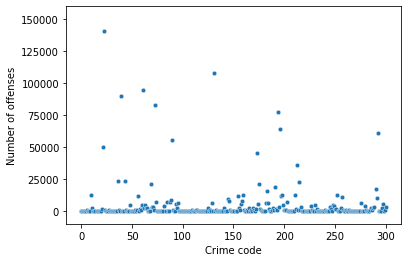
\includegraphics[width=\textwidth]{total-offenses-per-crime-full}
	\end{subfigure}\hfill
	\begin{subfigure}{0.45\textwidth}
		\centering
		\caption{Crimes with 5,000 offenses or less}
		\label{fig:total-offenses-per-crime-small}
		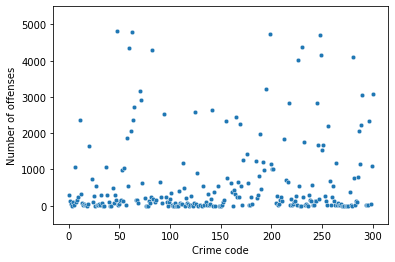
\includegraphics[width=\textwidth]{total-offenses-per-crime-small}
	\end{subfigure}
\end{figure*}

\begin{table*}
	\caption{Most notorious crimes and their occurrence in county 682. Column ``Total offenses'' is taken from \Cref{tab:notorious-crimes}. Column ``Contribution'' is the percentage of offenses that occur in county 682.}
	\label{tab:notorious-crimes-county}
	\centering
	\begin{tabular}{cccc}
		\hline\hline
		\\[-1.5ex]
		Crime code		&	Offenses in county 682	&	Total offenses		&	Contribution	\\[0.5ex]\hline
		\\[-1.5ex]
		131				&	84,952					&	108,031				&	78.63\%			\\[0.2ex]
		22				&	28,247					&	140,901				&	20.05\%			\\[0.2ex]
		61				&	24,101					&	\hspace{1ex}94,655	&	25.46\%			\\[0.2ex]
		73				&	23,743					&	\hspace{1ex}83,110	&	28.57\%			\\[0.2ex]
		39				&	21,698					&	\hspace{1ex}90,179	&	24.06\%			\\[0.5ex]
		\hline\hline
	\end{tabular}
\end{table*}

\begin{table*}
	\caption{Most notorious crimes and number of counties they occur in. Column ``Uniform contribution'' represents the contribution of each county if all occurrences where evenly distributed among counties.}
	\label{tab:notorious-crimes-uniform-distribution}
	\centering
	\begin{tabular}{ccc}
		\hline\hline
		\\[-1.5ex]
		Crime code		&	Number of different counties	&	Uniform contribution	\\[0.5ex]\hline
		\\[-1.5ex]
		131				&	\hspace{1ex}\,652				&	0.15\%			\\[0.2ex]
		22				&	1,228							&	0.08\%			\\[0.2ex]
		61				&	1,084							&	0.09\%			\\[0.2ex]
		73				&	1,099							&	0.09\%			\\[0.2ex]
		39				&	1,212							&	0.08\%			\\[0.5ex]
		\hline\hline
	\end{tabular}
\end{table*}

\begin{table*}
	\caption{Network descriptive statistics}
	\label{tab:network-details}
	\centering
	\begin{tabular}{rcc}
		\hline\hline
		\\[-1.5ex]
						&	With solo offenders	&	Without solo offenders	\\[0.5ex]\hline
		\\[-1.5ex]
		Total nodes		&	538,851				&	538,851			\\[0.2ex]
		Self edges		&	538,851				&	121,119			\\[0.2ex]
		Non-self edges	&	178,372				&	178,372			\\[0.2ex]
		Total edges		&	717,223				&	299,491			\\[0.5ex]
		\hline\hline
	\end{tabular}
\end{table*}

\begin{figure*}
	\caption{Degree distribution of the co-offending network. In panel (a), the degree distribution as a histogram. In panel (b), as smoothed discrete pdf.}
	\centering
	\label{fig:degree-distribution}
	\begin{subfigure}{0.48\textwidth}
		\centering
		\caption{Histogram}
		\label{fig:degree-distribution-bar}
		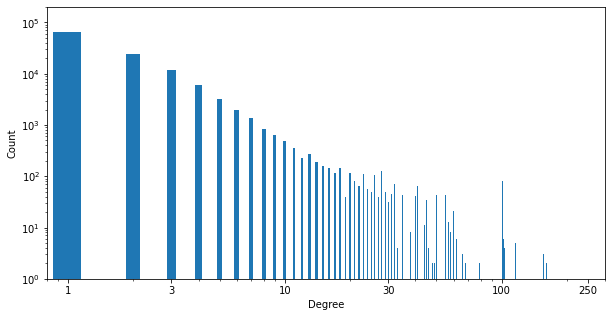
\includegraphics[width=\textwidth]{degree-distribution-bar}
	\end{subfigure}\hfill
	\begin{subfigure}{0.48\textwidth}
		\centering
		\caption{Smoothed discrete pdf}
		\label{fig:degree-distribution-line}
		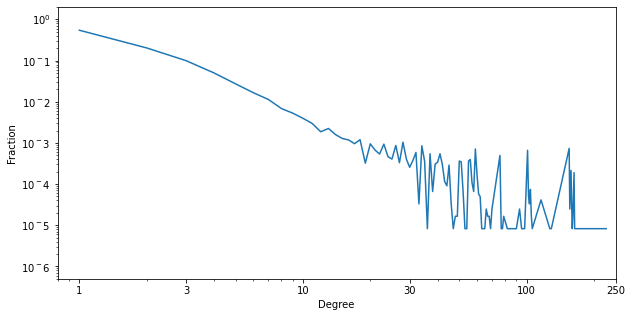
\includegraphics[width=\textwidth]{degree-distribution-line}
	\end{subfigure}
\end{figure*}

\begin{table*}
	\caption{Cumulative distribution of degree. Each row shows the number of nodes (and the percentage) that have at most degree $d$, for different values of $d$.}
	\label{tab:network-details}
	\centering
	\begin{tabular}{ccc}
		\hline\hline
		\\[-1.5ex]
		$d$		&	Number of nodes	&	Percentage	\\[0.5ex]\hline
		\\[-1.5ex]
		3		&	102,689			&	84.78\%		\\[0.2ex]
		5		&	112,042			&	92.51%		\\[0.2ex]
		10		&	117,373			&	178,372		\\[0.2ex]
		15		&	118,576			&	178,372		\\[0.2ex]
		20		&	119,134			&	178,372		\\[0.2ex]
		25		&	119,498			&	178,372		\\[0.2ex]
		30		&	119,849			&	299,491		\\[0.5ex]
		\hline\hline
	\end{tabular}
\end{table*}

\end{multicols}
\end{document}
